\documentclass[12pt,times,a4paper,twoside]{article}

\usepackage[utf8]{inputenc}	% Para caracteres en español
\usepackage[left=3cm,right=3cm,top=2cm,bottom=3cm]{geometry}
\usepackage{pagenote}

\usepackage{algorithm}
\usepackage{algorithmic}

\usepackage{amsmath,amsthm,amsfonts,amssymb,amscd}
\usepackage{mathtools,xparse}
\usepackage{mathrsfs}

\usepackage{multirow,booktabs}
\usepackage[table]{xcolor}
\usepackage{fullpage}
\usepackage{lastpage}
\usepackage{enumitem}
\usepackage{fancyhdr}

\usepackage{graphicx}
\usepackage{wrapfig}
\usepackage{setspace}
\usepackage{calc}
% \usepackage{color,soul}
\usepackage{multicol}
\usepackage{cancel}
\usepackage[retainorgcmds]{IEEEtrantools}
% \usepackage{xcolor} -- implied by xcolor

\usepackage{listings}
\usepackage{spverbatim}
\usepackage{fancyvrb}
\usepackage{hyperref}
\usepackage{float} 
\usepackage{natbib}

\usepackage{tikz}
\usepackage{pgfplots}
\usepackage{pgfplotstable}

\usepackage{soulutf8}
\usepackage{tabularx}

\usepackage[draft]{todo}
\newcommand{\fyTodo}[1]{\Todo[FY:]{\textcolor{orange}{#1}}}
\newcommand{\fyTodostar}[1]{\Todo*[FY:]{\textcolor{orange}{#1}}}
\newcommand{\fyDone}[1]{\done[FY]\Todo[FY:]{\textcolor{orange}{#1}}}
\newcommand{\fyDonestar}[1]{\done[FY]\Todo[FY:]{\textcolor{orange}{#1}}}

\colorlet{shadecolor}{orange!15}
\parindent 0in
\parskip 12pt
\geometry{margin=1in, headsep=0.25in}
\setlength{\belowdisplayskip}{8pt} \setlength{\belowdisplayshortskip}{8pt}
\setlength{\abovedisplayskip}{8pt} \setlength{\abovedisplayshortskip}{8pt}
\setlist{nosep}
\setlength{\parskip}{0.1cm}
\setlength{\parindent}{1em}

\theoremstyle{definition}
\newtheorem{defn}{Definition}
\newtheorem{lemma}{Lemma}[section]
\newtheorem{theorem}{Theorem}[section]
\newtheorem{proposition}{Proposition}[section]
\newtheorem{definition}{Definition}[section]
\DeclareMathOperator*{\argmax}{argmax}
\newcommand{\R}{\ensuremath{\mathbb{R}}}

\pgfkeys{
    /tr/rowfilter/.style 2 args={
        /pgfplots/x filter/.append code={
            \edef\arga{\thisrow{#1}}
            \edef\argb{#2}
            \ifx\arga\argb
            \else
                \def\pgfmathresult{}
            \fi
        }
    }
}

\DeclarePairedDelimiter{\abs}{\lvert}{\rvert}
\DeclarePairedDelimiter{\norm}{\lVert}{\rVert}
\NewDocumentCommand{\normL}{ s O{} m }{%
  \IfBooleanTF{#1}{\norm*{#3}}{\norm[#2]{#3}}_{L_1}%
}

\title{Combination of generic and specific layers in multidomain learning}
\author{}
\date{}

\begin{document}

\maketitle
\begin{center}
{\LARGE \bf}\fyDone{Make a proper title}
\end{center}

\section*{Word Level Adaptive Domain Adaptation}
We consider a generic encoder-decoder architecture for a multi-domain sequence to sequence learning. Let $h \in \R^d$ the output of the encoder, \cite{} proposes to use an adapted representation for domain $k$ defined as $h' = h + a_k(h)$. This means that all words in all sentences in domain $k$ will use the adapter module represented by $a_k$. In a multilayer version with highway connections (see Figure~\ref{fig:hrl-architecture}), $a_k(h) = \sum_{l} a_{kl}(h^l)$ where $h^l$ is the distributed representation of the sequence at the $l^{th}$ layer.

\begin{figure}[h!]
  \centering
  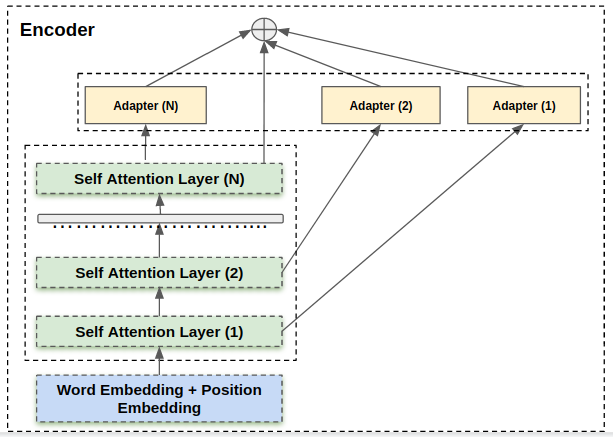
\includegraphics[scale=0.5]{fig/highway_residual}
  \caption{Highway multi-domain network with residual layers}
\label{fig:hrl-architecture}
\end{figure}

 A ``gated'' version uses $h' = h + a_k(h) \odot{} z_k(h)$\footnote{Or $a_k(h) = \sum_{l} a_{kl}(h)$, where the summation runs over layers, see Figure~\ref{fig:hrl-architecture}} \fyDone{$a_k(h)=$ somme tous les composants résiduels} where $z_k$ is a function of $h$ taking values in $[0,1]$. More precisely, $h$ and $h'$ are sequences of context vectors and the combination is performed element-wise, yielding:\fyDone{pourquoi pas gating: $(1-a_k(h(w))*hh(w)$ ? Notation mult. component wise ?}

\begin{equation}
   \forall t \in [1 \dots{} T], h'(w_t) = h(w_t) + a_k(h(w_t)) \odot{} z_k(h(w_t)). \label{eq:gated-residual}
\end{equation}
 
In Word Level Adaptive Domain Adaptation (WADA), $z_k(h(w))$ is designed to reflect the ``topicality'' of  word $w$ is in domain $k$: the more likely $w$ is in domain $k$, the larger $z_k(h(w))$ should be. Word-level adaptive domain adaptation aims to reduce the variation caused by $a_k$ to the adapted context vector $h'$ (compared to $h$) for words that are not typical of domain $k$. For a domain, there are 2 types of non-topical words: out-of-domain words that rarely or never appear in the in-domain texts and frequent words that appear equally frequently in many domains. \fyTodo{This is like a poor Tf-idf - can be because tf is small or because idf is small} 

\fyTodo{Experiment: compute posterior probability of words that have poor $tf-idf$ to verify the gating operation}. 

By reusing the learned generic representation for non-topical words, we can bound the risk of poor predictions in case of out-of-domain words by the risk of the learned generic model (see below).

\section*{The training process}
The training process comprises three main steps:
\begin{enumerate}
\item Pretraining a generic model with a mixed corpora comprising data from multiple domains;
\item Training a domain classifier on top of the encoder and decoder; during this step, the parameters of the generic model are frozen. This model computes the posterior domain probability $p(k|h(w_t))$ for each word $w_t$ based on the representation computed by the last layer.
  
  Domain classifiers take as input the output of the encoder and the output of the decoder, i.e at the last self-attention layer of the encoder and the attention layer of the decoder. \fyDone{Next sentence is a repetition}
  % Two classifiers are placed respectively on top of the last encoder and decoder layers:
  \begin{align}
    \forall t \in [1 \dots T], h_{enc}(w^{src}_t) = Enc(x)(w^{src}_t), z^{enc}_k(w^{src}_t) = p(k| h^{enc}(w^{src}_t))
  \end{align}
  \fyTodo{what are x and y ?}
  and
  \begin{align}
    h_{dec}(w^{tgt}_t)=Dec(x, y_{i<t})(w^{tgt}_t)  z^{dec}_k(w^{tgt}_t) = p(d=k| h_{dec}(w^{tgt}_t))
  \end{align}
  Where x is source sentence, y is target sentence, $x=\lbrace w^{src}_0,..,w^{src}_{T_0}\rbrace$, $y=\lbrace w^{tgt}_0,..,w^{tgt}_{T_1} \rbrace$
  
\item Training the parameters of adapters with in-domain data separately for each domain while freezing the parameters of the generic model and of the domain classifiers.
\end{enumerate}

During inference, $z_k$ is used to regulate the strength of the adapter module as suggested in equation~\ref{eq:gated-residual}.

\section*{Weakness of the method}

This method\fyTodo{Do not start with the weaknesses} depends crucially to the quality of the classifier $p(k|h(w))$. Moreover, the classifier can fail to detect in-domain words in the case of polysemous words. For example, the word "joint" in ``joint stereo'', ``joint sprain'' and ``joint project'' correspond to multiple translations such as "joint" and "articulaire" in French. In the unbalanced dataset as the mixed corpora (6 in-domain corpora),  "joint stereo" is hardly to be detected as in IT domain, therefore "joint stereo" does not profit the finetuning's effect even being translated with the adapters of IT domain.

\section*{Analysis on the risk of new method}

Recall that the combination of a generic representation and a residual adapter introduced in \citep{BapnaXX} is defined as:
\begin{equation}
  h' = h + a_k(h) \label{eq:residual-adapter},
\end{equation}

where $h \in \R^{d_{model}}$ is the output of shared ``generic'' layers, i.e $h=M(x,y)$, $M: \mathbb{X} \times \mathbb{Y} \rightarrow \mathbf{\Omega}\subset \R^{d_{model}}$, $a_k$ is the residual adapter defined as a function $a_k: \R^{d_{model}} \rightarrow \R^{d_{model}}$.\fyTodo{$\R^d$ might be enough.}

The poor performance of fine-tuned models with a residual layer happens when the value of $a_k(h)$ of an out-of-domain example $(x^{adv}, y^{adv})$ is adversarial to the model. Indeed, by fine-tuning the adapter with only in-domain data, $a_k$ never encounters adversarial examples, which makes it error-prone in the face of out-of-domain examples. The intuition of WADA is that by controlling the weight of $a_k(h)$ in the combination, we can hope to reduce the wrong impact of $a_k$ on adversarial examples. To implement this idea, we  investigate a convex combination\fyDone{Entre $h$ et $h + a h$} of the generic and the residual layers and define the adapted representation of a training sample from domain $k$ as: \fyTodo{Use real labels in equation}

\begin{equation}
  h' = h + a_k(h) \odot f(z_k), 
\label{eq:2}
\end{equation}

\noindent{}where
\begin{itemize}
\item $z_k = p(d=k | h=M(x,y)) = p_k(h)$ with $p: \mathbf{\Omega} \rightarrow \mathbf{\Delta}^{K}$\fyTodo{This is an overkill}. In the sequence to sequence version, there are 2 classifiers which are placed respectively on top of the encoder and of the decoder.
$z^{enc}_k(w_t) = p(d=k| h_{enc}(w_t)=Enc(x)(w_t))$ and $z^{dec}_k(w_t) = p(d=k| h_{dec}(w_t)=Dec(y_t,x,y_{i<t})(w_t))$
\fyTodo{Attention à $x$ et $y$}
\item f is an activation function $f: [0,1] \rightarrow [0,1]$.
\end{itemize}

We assume that the hidden distribution of a multi-domain problem limited to an unknown mixture of $K$ in-domain distribution, i.e, $$\mathcal{D}(x,y) = \sum_{k=1}^{K} P(d=k) P(x,y|d=k)$$. We denote also $\mathcal{D}_k$ the data distribution for domain $k$: $\mathcal{D}_k = P(x,y|d=k)$.

We define some important constants:
\begin{itemize}
\item Inseparability of domains over a fixed representation space $\Omega$\fyTodo{ugly equation, is my version better ?}
\begin{align}
  \varepsilon_{insep} =& \min_{p} \sum_{k\in[1..K]} \mathbb{E}_{x,y \sim \sum_{i\in [1..K]} \mathcal{D}_{i}*p(d=i)}(\mathbf{1}_{d\neq k} p(k|h)) \\
  \varepsilon_{insep} =& \sum_{k=1}^K P(k)  \mathbb{E}_{x,y \sim \mathcal{D}_k} (\sum_{k' \neq k} P(k'|x,y))
\end{align}

\fyTodo{This does not depend on anything, this is how are data is but we can not know it} 
\item Inseparability of domain $k$ from other domains over a fixed representation space $\Omega$
  \begin{align}
    \varepsilon_{insep}(k) &= \min_{p} \mathbb{E}_{x,y \sim \sum_{i\in [1..K]} \mathcal{D}_{i}*p(d=i)}(\mathbf{1}_{d\neq k} p(k|h)) \\
    \varepsilon_{insep}(k) &= \mathbb{E}_{x,y \sim \mathcal{D}_k} (\sum_{k' \neq k} P(k'|x,y))    
  \end{align}
\item Risk of the generic model: $$R = \mathbb{E}_{x,y \sim\mathcal{D}}(l(h = M(x, y_{<t}), y_t))$$.\fyDone{wrt to which distribution ?}\fyTodo{is $x$ a sequence ? then we need to sum over $t$ to get the loss}
\item $\mathbf{\Omega_{k,p_{0}}} = \lbrace h | z_k = p_\theta(k|h) < p_0\rbrace$.
\item Risk of the adapted model for the in-domain test set:\fyTodo{Use same notations as before}
  $$R_k = \mathbb{E}_{x,y \sim \mathcal{D}_k} [l(h + a_k(h) \odot f(z_k), y)]$$.
\end{itemize}

We also need two assumptions on the regularity of the activation and the loss functions:\fyTodo{Are these standard in such models - if yes, cite}
\begin{itemize}
\item $a_k$ is bounded in sense of $\normL{a_k(h)} < M$\fyTodo{$M$ is already used}
\item the loss function is bounded:  $l(h,y) < A, \forall h \in \Omega + \mathbb{B}(M)$, where $\mathbb{B}(M)=\lbrace x\in \mathbb{R}^{d_{model}} | \normL{x}<M \rbrace$. We note $A +_{\alpha}B = \lbrace x+ \alpha y  | \alpha \in [0 \in 1], x \in A, y \in B \rbrace$ \fyTodo{Notation $A$ is a scalar, not a set}
  $\forall x,y$
\end{itemize}

Finally, we assume that our domain classifier $P_\theta$ is good enough, i.e that\fyDone{Attention à $p$}
$$\exists \gamma, \forall k, err(k, \theta) = \mathbb{E}_{x,y \sim \mathcal{D}_{k}} \sum_{k' \neq k} p_\theta(k'|h=M(x,y)) < \varepsilon_{insep}(k) + \gamma$$ with $\gamma$ sufficiently small.
We then evaluate the risk of the model adapted to domain $smallk$ with residuals $a_k$ for arbitrary examples from $K$ domains:\fyTodo{(x,y) is sampled from some distribution}
\begin{equation}
\begin{split}
  R(M,a_k) &= \mathbb{E}_{(x,y) \sim \mathcal{D}}[l(h + a_k(h) \odot f(z_k),y)] \\
  &= \mathbb{E}_{(x,y) \sim \mathcal{D}}[l(h + a_k(h) \odot f(z_k),y)\mathbf{1}_{\mathbf{\Omega_{k,p_{0}}}}(h)] + \\
  &\quad + \mathbb{E}_{(x,y) \sim \mathcal{D}}[l(h + a_k(h) \odot f(z_k),y) \mathbf{1}_{\mathbf{\Omega_{k,p_{0}}^{c}}}(h)]
\end{split}
\end{equation}

By designing a suitable activation function, we can map $f: [0,p_{0}] \rightarrow [0,\delta]$. Then with $\delta$ is small enough we can have an approximation of the first term:\fyTodo{We need $l$ to be smooth here, no ?}
\begin{align*}
  \mathbb{E}_{x,y \sim \mathcal{D}}[l(h + a_k(h) \odot f(z_k),y)\mathbf{1}_{\mathbf{\Omega_{k,p_{0}}}}(h)] \approx{}&
                                                                                                                      \mathbb{E}_{x,y \sim \mathcal{D}}[l(h,y)\mathbf{1}_\mathbf{\Omega_{k,p_{0}}}(h)] \\
  \leq& \mathbb{E}_{x,y \sim \mathcal{D}}[l(h,y)] = R
\label{eq:4}
\end{align*}
The second term: $ L(M,a_k) = \mathbb{E}_{x,y \sim \mathcal{D}}[l(h + a_k(h) * f(z_k),y) \mathbf{1}_{\mathbf{\Omega_{k,p_{0}}^{c}}}(h)]$ can be bounded as follows:
\begin{equation*}
\begin{split}
L(M,a_k) &= \displaystyle{\mathop{\sum}_{k'}\mathbb{E}_{x,y \sim \mathcal{D}_{k'}}[l(h } + a_k(h) * f(z_k),y) * \mathbf{1}_{\mathbf{\Omega_{k,p_{0}}^{c}}}(h)]p(d=k') \\
	& \leq \displaystyle{\mathop{\sum}_{k' \neq k}} A * \mathbb{E}_{x,y \sim \mathcal{D}_{k'}} [\mathbf{1}_{\mathbf{\Omega_{k,p_{0}}^{c}}}(h)]P(d=k') \\
	& \quad + \mathbb{E}_{x,y \sim \mathcal{D}_k}[l(h + a_k(h) * f(z_k),y) * \mathbf{1}_{\mathbf{\Omega_{k,p_{0}}^{c}}}(h)]P(d=k) \\
	&\leq A * \frac{\mathbb{\varepsilon}_{insep}^k + \gamma}{p_{0}} + R_k * P(d=k)
\end{split}
\label{eq:5}
\end{equation*}

The last inequality is verified since:
\begin{equation}
\begin{split}
\displaystyle{\mathop{\sum}_{k' \neq k}} A * \mathbb{E}_{x,y \sim \mathcal{D}_{k'}} [\mathbf{1}_{\mathbf{\Omega_{k,p_{0}}^{c}}} (h)]P(d=k') &\leq A * \displaystyle{\mathop{\sum}_{k' \neq k}} \mathbb{E}_{x,y \sim \mathcal{D}_{k'} } [\frac{p_k(h)}{p_0}]P(d=k') \\
		& = \frac{A}{p_0} \mathbb{E}[\mathbf{1}_{d\neq k}p_k(h)] \\
		& \leq \frac{A}{p_0} (\mathbb{\varepsilon}_{insep}^k + \gamma)
\end{split}
\end{equation}
because
$$ \mathbf{1}_{\mathbf{\Omega_{k,p_{0}}^{c}}}(h) \leq \frac{p_k(h)}{p_0} $$
Combining inequalities \ref{eq:4} and \ref{eq:5} we obtain the risk in general case of the adapted model $(M,a_k)$ $$R(M,a_k) \leq R + A * \frac{\mathbb{\varepsilon}_{insep}^k + \gamma}{p_0} + P(d=k)R_k$$

If we consider the original version of the residual adapter, with the same assumption in the regularization of the adapter, the bound of the risk of translating out-of-domain (the second term in the inequality above) is only $A$ (the bound of loss function). By using an adaptive version, we reduce A by factor $\frac{p_0}{\epsilon^k_{insep}+\gamma}$, which is high if we choose $p_0$ is high enough, the domains are distant in the fixed representation space and the classifier is good enough. 

\end{document}


